\section{Genetic Algorithm Implementation in Python}

This section describes the implementation of a genetic algorithm in Python.

\subsection{The Basics}

The traveling salesman problem assumes that each city can be reached from any other city; that is, the graph is fully connected. This graph can be very simply represented as a Python list of vertices where the value is each vertex's XY coordinate. Because every vertex connects to every other, we can implicitly assume that each edge (u, v) exists, and that it's value is the simple Euclidean distance between the vertices. As such, the fully connected graph can be represented as a simple list of XY tuples.

\begin{figure}[H]
\begin{python}
FullyConnectedGraph = [(0.1313626194361659, 0.9537494015311131
 (0.6931250094496763, 0.042877414320216856
 (0.17355376046059656, 0.41488071009395744
 (0.47339225625323855, 0.9527742641692806
 (0.399394375477357, 0.6665748105617455
 (0.43170810077728095, 0.13591355449019749
 (0.6351099070806486, 0.5983664092055496
 (0.8957003084360835, 0.656752235127581
 (0.7658498920971735, 0.6465721898932276
 (0.8026020533786447, 0.06444102480533265)]
\end{python}
\caption{A simplified representation of a random fully connected graph with N=10. }
\end{figure}

We can visualize this fully connected graph in 2D space, and plot each edge. 

\begin{figure}[H]
\centering
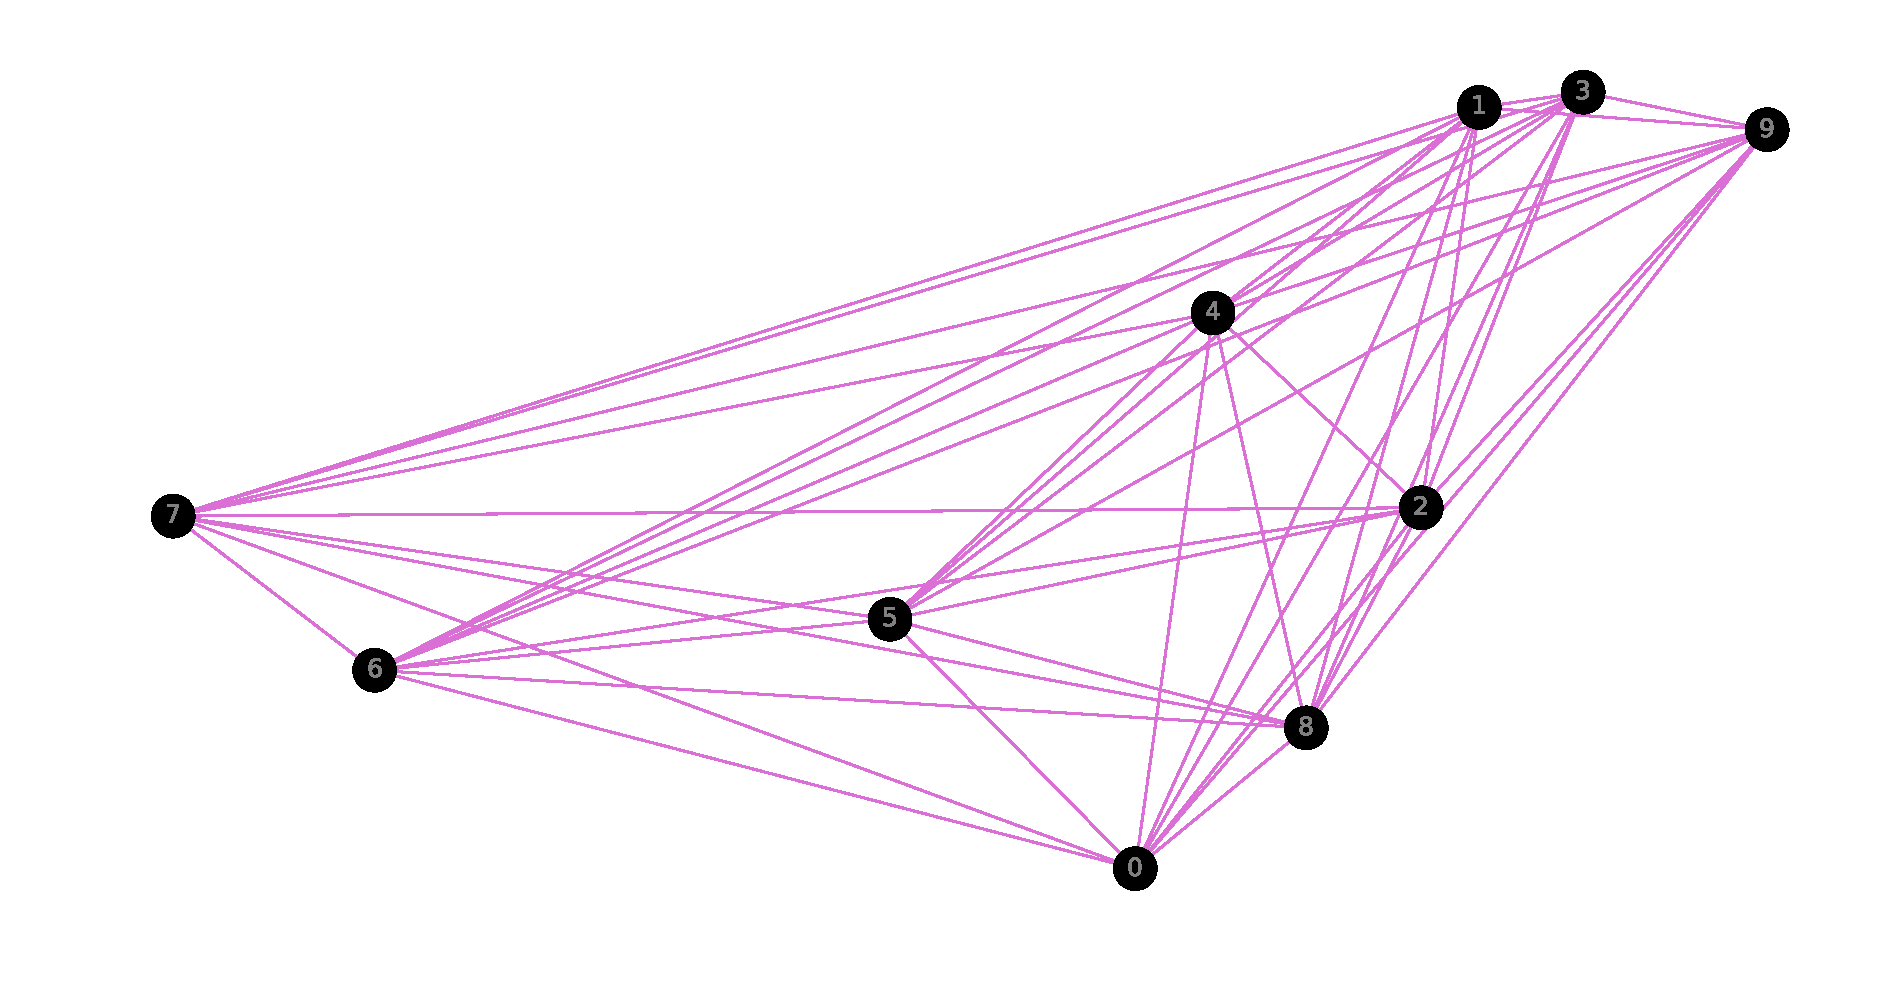
\includegraphics[width=2in]{images/fully_connected_graph.eps}
\caption{A fully-connected graph with 10 vertices, each placed at random XY coordinates. Each vertex represents a city, and the edge weights are the Euclidean distance between the cities.}
\end{figure}

Any valid solution to the problem is simply a permutation of the list of vertices. For simplicity, we will number the vertices from 0 to N. For example, for a graph with 10 vertices, any of the following are valid solutions:

\begin{figure}[H]
\begin{python}
[2, 3, 4, 8, 9, 6, 1, 5, 7, 0]
[8, 0, 6, 2, 4, 3, 1, 9, 5, 7]
[9, 0, 5, 3, 7, 4, 8, 6, 1, 2]
\end{python}
\caption{Three valid solutions to the traveling salesman problem with cities numbered 0 to N-1. Each is a permutation of the array 0..10.}
\end{figure}

This is a visualization of a single solution.

\begin{figure}[H]
\centering
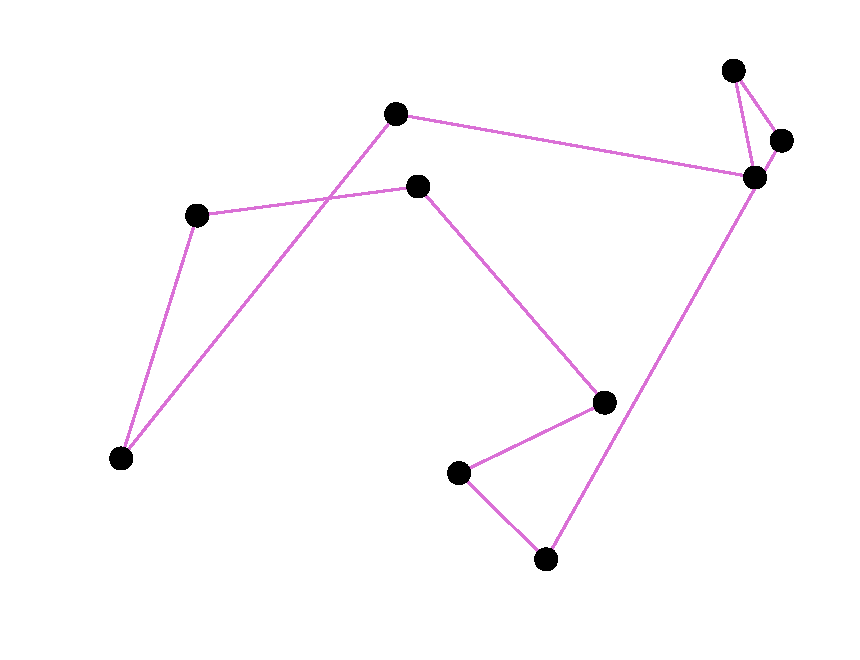
\includegraphics[width=2in]{images/single_solution.eps}
\caption{An instance of a possible solution to the traveling salesman problem with N=10.}
\end{figure}

To compute the fitness of a solution, the total distance of the journey is measured, by walking through the path one edge at a time, eventually looping back to the starting point.

\begin{figure}[H]
\begin{python}
def compute_fitness(self):
  total_dist = 0
  # Compute the fitness, edge by edge
  for i in range(len(self)):
    edge_start = self.get(i)
    edge_end = self.get((i+1)%len(self)) 
    total_dist += self.graph.dist_between(edge_start, edge_end)
  self.fitness = total_dist
  return self.fitness
\end{python}
\end{figure}

\subsection{Creating the First Generation}

The first step in a genetic algorithm is to create a first chromosome, using random solutions. This is straightforward, because a random solution is simply a permutation of the list 0..N. Here, we create a range of numbers sorted from 0 to N, and use the random module to randomly shuffle it. This process is repeated for as many solutions are desired in each chromosome.

\begin{figure}[H]
\begin{python}
# Create random solutions to seed the algorithm.
def generate_random_chromosomes(self):
  for i in range(self.num_chromosomes):
    arr = range(self.graph.num_nodes)  # Begin with the solution 0, .. N-1
    random.shuffle(arr)         # Shake it up to make a random solution
    self.current_generation.append(Solution(arr, self.graph))
\end{python}
\end{figure}
 	
\subsection{Selection}

The goal of selection is to select a group of individuals from the current generation to begin the process of creating the next generation. The process aims to predominantly select the fittest individuals, but allow for less fit individuals to also survive on occasion, to preserve diversity. A good approach for this is a `tournament' selection. In tournament selection, a random batch of four individuals are chosen from the current generation. The fittest is then placed into the next generation. This is repeated until the next generation is full. Using a small selection group -- in this case, only four -- ensures diversity while favoring the top quartile of fittest solutions. 

\begin{figure}[H]
\begin{python}
  # Use a "tournament select" to choose winning parents.
  # Repeatedly pick 4 random elements and put the 
  # best one into the next into the next generation.
  def select_next_generation(self):
    self.next_generation = []

    # Compute all of the fitnesses so we can run tournaments.
    self.compute_all_current_gen_fitnesses()

    # Fill the next generation with tournament winners
    while len(self.next_generation) < len(self.current_generation
      # Choose four random solutions
      sample = random.sample(self.current_generation, 4)
      # Pick the winner (lower fitness value is best)
      fittest = min(sample, key=lambda x: x.fitness)
      self.next_generation.append(fittest)	
\end{python}
\end{figure}

\subsection{Crossing Over}

Crossing first groups each of the newly selected next generation into pairs, which I refer to as `mom' and `dad'. In crossing over, the algorithm merges a bit of each solution into the other.

We do this by first starting with mom. We take a random chunk of mom's solution and insert it into a new array at the same location. We then insert dad's solution into the new array. This is complex because we aim to retain dad's solution order as much as possible, without duplicating any of the vertices (which is invalid). The procedure cross\_merge\_array below does this by inserting dad's solution into the new array, element by element, unless that element was already inserted as part of crossing-over. This procedure is repeated for both parents, and then repeated for every pair of parents. 

\begin{figure}[H]
\begin{python}
# Uses ordered crossover to cross two arrays.
def cross_merge_arr(self, parent1, parent2):

  # First choose two random indices in parent1 to select the crossover section.
  crossover_points = sorted(random.sample(parent1, 2))
  
  # Extract that section of parent1 and store it in a hashset for quick lookups
  crossover = parent1[crossover_points[0]:crossover_points[1]]
  crossover_set = set(crossover)                
  
  # Now push the crossover into an empty output array at the same indices
  out_arr = [None] * self.graph.num_nodes
  out_arr[crossover_points[0]:crossover_points[1]] = crossover

  # Fill in the rest of output array from parent2, maintaining parent2's order.
  # Iterate over parent2's nodes.
  # Attempt to insert each node into the output array. 
  # If the slot is empty, AND the node isn't in the crossover set, insert into output array.
  # Otherwise, try to place it in the next slot.
  placement_index = 0
  for item in parent2:
    while placement_index < self.graph.num_nodes and out_arr[placement_index] != None:
      placement_index += 1
    if item not in crossover_set:
      out_arr[placement_index] = item
      placement_index += 1
  return out_arr
\end{python} 
\end{figure}

\subsection{Mutation}

The final step of the genetic algorithm is mutation. Mutation is intended to create a bit of randomness to help the solutions occasionally find brand new paths. The key constraint on mutation is that it must still yield an acceptable solution, that is, a solution where each vertex is visited exactly once. A good way to ensure that is to simply swap two vertices in the solution.

\begin{figure}[H]
\begin{python}
# Mutate chromosomes by two swapping random elements at the mutation rate.
# Swapping maintains the solution integrity 
# (ensuring no node is visited twice or not visited).
def mutate(self):
  for solution in self.next_generation:
  # Each chromosome has a chance of mutation
    if random.random() < self.mutation_rate: 
      index_a = random.randrange(0, self.graph.num_nodes)
      index_b = random.randrange(0, self.graph.num_nodes)
      solution.swap(index_a, index_b)
\end{python}
\end{figure}